

%\documentclass[a4paper]{jarticle}


\section{msankey.rb Draw sankey diagram\label{sect:msankey}}
\index{msankey@msankey}

The sankey diagram is a technique to visualize Directed Acyclic Graph (DAG), in which the weight of edge is defined in proportion with the flow quantity between contact points. The diagram is typically used to visualize energy transfer between processes in power transmission network. 

This visualization command calls to internal D3 library (Data-Driven Documents) to generate sankey diagrams (\url{http://bost.ocks.org/mike/sankey/}).   

The input data is shown in Table \ref{tbl:sankey_input1}, each edge and node pair and their corresponding value are shown in a row as CSV data. The sankey diagram is generated as one html file which can be displayed in the browser as shown in diagram (\ref{fig:sankey1}).  

The orientation of the graph starts from left to right, the first item specified at command parameter \verb|f=| corresponds to the left, and the second item corresponds to the right. 
The color bar corresponds to the node, and the edge corresponds to the connecting points.  
Interval relaxation method is used to determine the output position of the node.
For more details, please refer to the original URL above.
Based on experiments, it consumes more time to draw 5 nodes $\times$ 10 level positions $=50$ nodes. 

In order to use this command, json library in nysol/mcmd library is required.


\begin{table}[htbp]
\begin{center}
\begin{tabular}{c}

\begin{minipage}{0.12\hsize}
\begin{center}
\caption{Input data (Closed walk directed graph)\label{tbl:sankey_input1}}
{\small
\begin{tabular}{cccc}
\hline
node1&node2&val\\
\hline
a&b&1\\
a&c&2\\
a&d&1\\
b&c&3\\
b&d&3\\
c&f&1\\
c&e&4\\
d&e&1\\
e&f&3\\
\hline
\end{tabular} 
}
\end{center}
\end{minipage}

\end{tabular} 
\end{center}
\end{table} 


\begin{figure}[htbp]
\begin{center}
\begin{tabular}{c}

\begin{minipage}{0.5\hsize}
\begin{center}
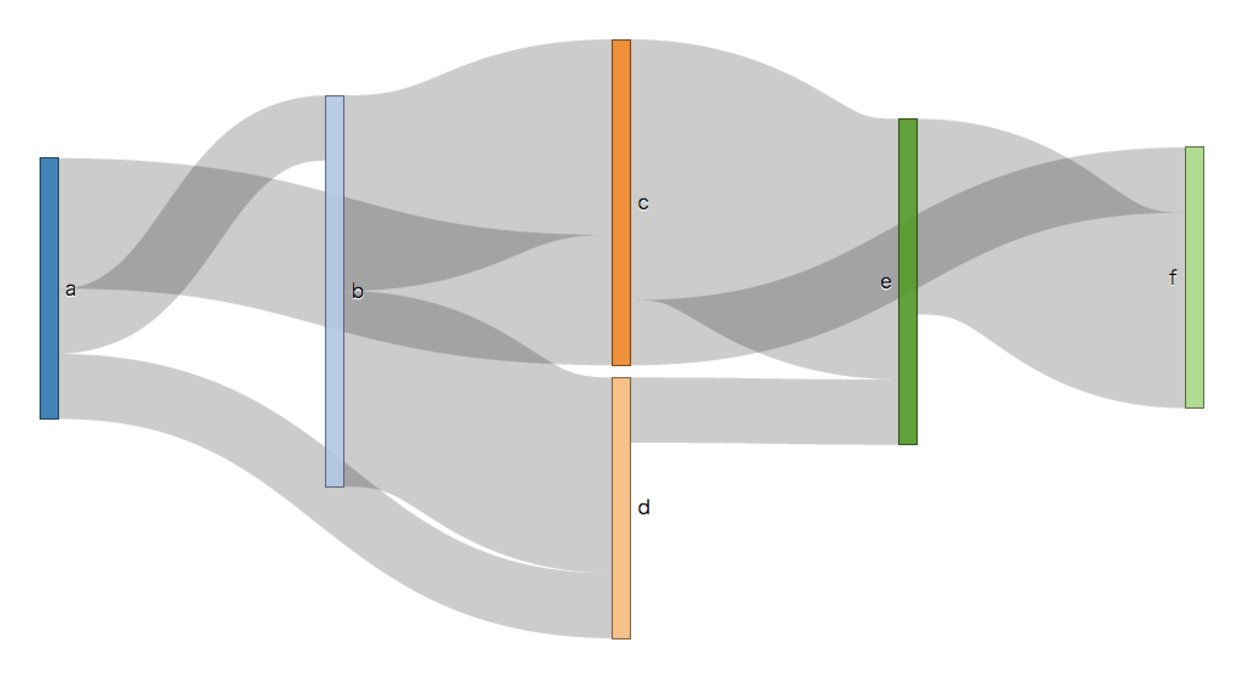
\includegraphics[scale=0.5]{figure/sankey1.eps}
\caption{Sankey diagram \label{fig:sankey1}}
\end{center}
\end{minipage}

\end{tabular}
\end{center}
\end{figure}



\subsection{Format}
\begin{verbatim}
msankey [i=] f= v= [o=] [t=] [T=] [--help]
\end{verbatim}

\begin{table}[htbp]
{\small
\begin{tabular}{ll}
\verb|i=| & : Edge data file   \\
\verb|f=| & : Two node field names on edge data \\
\verb|v=| & : Field name of edge weight  \\
\verb|o=| & : Output file (HTML file) \\
\verb|t=| & : Specify title  \\

\verb|-T| & : Working directory (default:/tmp) \\
\verb|--help| & : Show help \\
\end{tabular} 
}
\end{table} 

\subsection{Example}
\subsubsection*{例1: 基本例}

前節の解説で用いてる例。


\begin{Verbatim}[baselinestretch=0.7,frame=single]
$ more dat1.csv
node1,node2,val
a,b,1
a,c,2
a,d,1
b,c,3
b,d,3
c,f,1
c,e,4
d,e,1
e,f,3
$ msankey.rb i=dat1.csv f=node1,node2 v=val o=output.html
$ head output.html
<!DOCTYPE html>
<html class="ocks-org do-not-copy">
<meta charset="utf-8">
<!--
<title>Sankey Diagram</title>
-->
<title></title>
<style>
\end{Verbatim}


%\end{document}

